\documentclass[titlepage,a4paper]{article}
%¿como llegaste a esto si te estamos entregando un PDF?, igualmente, es un muy lindo informe y yo creo que merece un 10 por el esfuerzo y la prolijidad
%el liberalismo es la solución
%ANDY LA CONCHA DE TU MADRE
\usepackage{a4wide}
\usepackage[colorlinks=true,linkcolor=black,urlcolor=blue,bookmarksopen=true]{hyperref}
\usepackage{bookmark}
\usepackage{fancyhdr}
\usepackage[spanish]{babel}
\usepackage[utf8]{inputenc}
\usepackage[T1]{fontenc}
\usepackage{graphicx}
\usepackage{float}
\usepackage{multicol}
%liberalismo
\usepackage{minted} %codigo
%liberalismo
\pagestyle{fancy} % Encabezado y pie de página
\fancyhf{}
\fancyhead[L]{TP1 - Grupo 1}
\fancyhead[R]{Análisis Numérico - FIUBA}
\renewcommand{\headrulewidth}{0.4pt}
\fancyfoot[C]{\thepage}
\renewcommand{\footrulewidth}{0.4pt}
\usepackage[utf8]{inputenc}
%viva perón liberal
%abajo el comunismo
\begin{document}
\begin{titlepage} % Carátula
	\hfill
\includegraphics[width=6cm]{logofiuba.jpg}
    \centering
    \vfill
    \Huge \textbf{Trabajo Práctico 1}
    \vskip2cm
    \Large [ 75.12 - 95.04 ] Análisis Numérico\\
    Curso 5 \\ 
    Primer cuatrimestre de 2020\\
    \vfill
    \begin{tabular}{ | l | l | } % completen con padron, LOL ya estaba completo
      \hline
        De Angelis Riva, Lukas & 103784 \\ \hline
        Gomez, Joaquín & 103735 \\ \hline
        Grassano, Bruno & 103855 \\ \hline
        Guillemi, Andrés & 104006\\ \hline 
        Rodriguez, Ezequiel & 103976 \\ \hline
        Romero, Adrián & 103371 \\ \hline
  	\end{tabular}
    \vfill
    \vfill
    \vfill
\end{titlepage}

\tableofcontents % Índice general
\newpage

\section{Introducción}\label{sec:intro}
En este trabajo práctico creamos un programa para la búsqueda de raíces de funciones a través de los siguientes métodos numéricos aprendidos en la materia:
\begin{itemize}
    \item Bisección
    \item Newton-Raphson
    \item Newton-Raphson modificado
    \item Secante
\end{itemize}


Con este fin, primero graficamos las funciones en Geogebra para tener una idea sobre ellas, corroborando que los intervalos brindados en el enunciado eran válidos para los métodos. Luego, obtenemos las raíces y con la historia de los resultados pasamos a analizar los distintos métodos analizando los ordenes de convergencia, su conveniencia en tiempos de cómputo y error en el resultado.

Para verificar los resultados, calculamos las raíces mediante la biblioteca de Python `SciPy`. De esta manera pudimos corroborar el correcto funcionamiento de las funciones programadas.

\section{Objetivos}\label{sec:objetivos}
El objetivo del trabajo práctico es obtener la raíz de las tres funciones dadas mediante los métodos numéricos indicados, para luego analizar el orden de convergencia P y la constante asintótica de cada método. $\lambda$


\section{Gráficos de las funciones}\label{sec:graficosfun}

\begin{figure}[H]
\centering
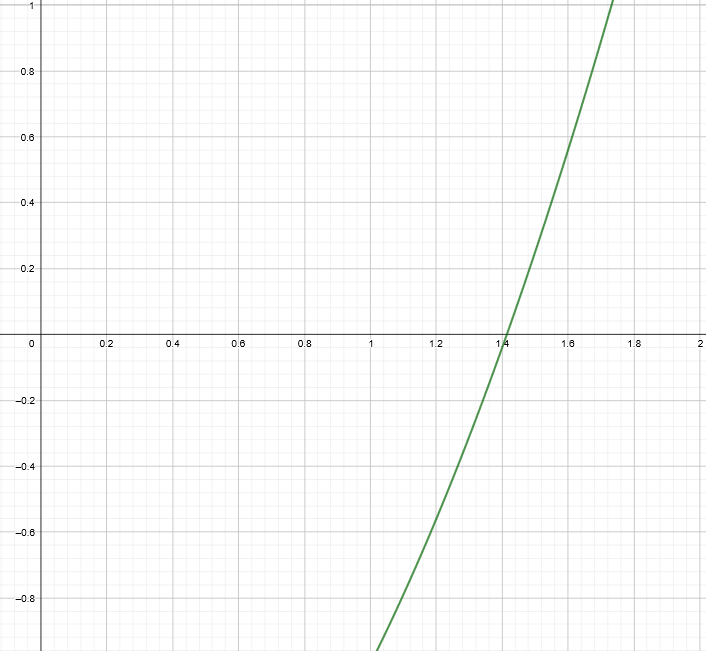
\includegraphics[width=0.8\textwidth]{funcion1.png}
\caption{\label{fig:class01}Gráfico correspondiente a la primera función en el intervalo [0;2].}
\end{figure}

\begin{figure}[H]
\centering
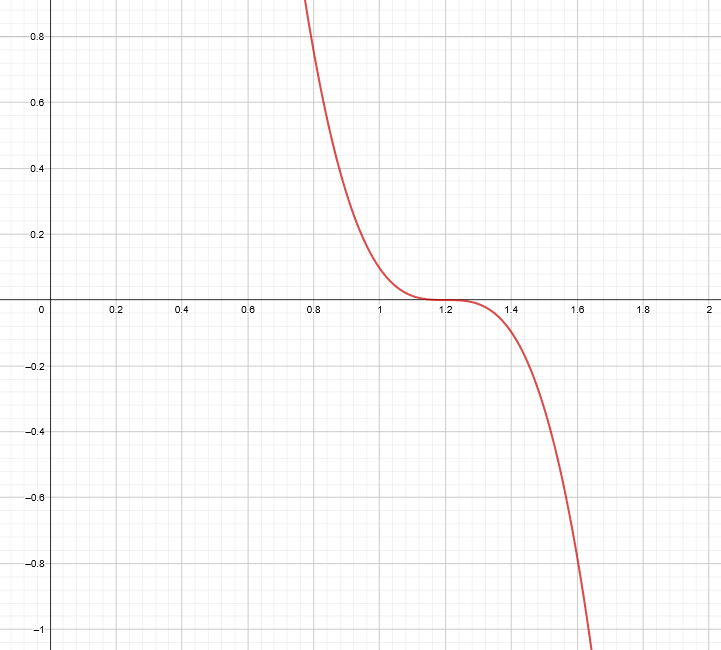
\includegraphics[width=0.8\textwidth]{funcion2.png}
\caption{\label{fig:class01}Gráfico correspondiente a la segunda función en el intervalo [0;2].}
\end{figure}

\begin{figure}[H]
\centering
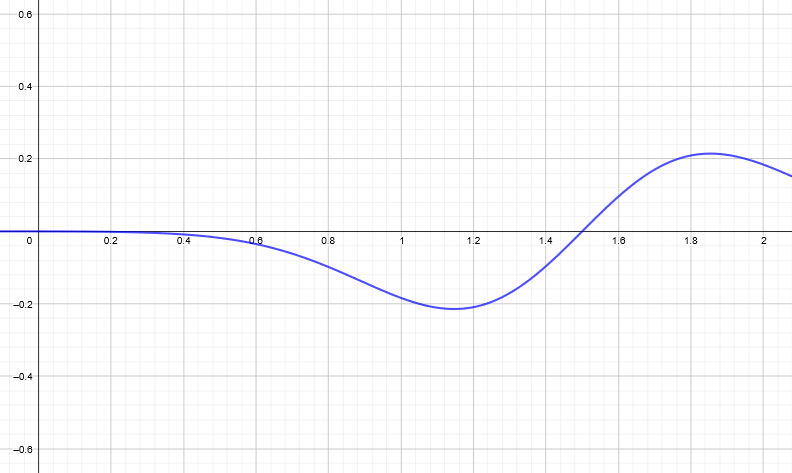
\includegraphics[width=0.8\textwidth]{funcion3.png}
\caption{\label{fig:class01}Gráfico correspondiente a la tercera función en el intervalo [0;2].}
\end{figure}

\section{Búsqueda de raíces}\label{sec:busqueda_raices}

\subsection{Bisección}\label{sec:biseccion}
El método de bisección halla la raíz mediante la siguiente fórmula por métodos iterativos hasta que 
$ |p_{n+1} - p_{n}| < \mbox{$\epsilon$} $ , tomando los límites iniciales de intervalo ${a_n}$ y ${b_n}$:

\smallskip

$\mbox{Sea }p_n = \frac{a_n+b_n}{2}\mbox{, entonces, en la siguiente iteración}$
\begin{center}
    $
    \quad a_{n+1} =\left\{ \begin{array}{lcc}
                 a_n & \mbox{si } f(a_n)\cdot f(r_n) <0 \\
                 \\ p_n & \mbox{si } f(a_n)\cdot f(r_n) > 0 \\
                 \end{array}
       \right. 
    $
    $
    \quad b_{n+1} =\left\{ \begin{array}{lcc}
                 b_n & \mbox{ si } f(b_n)\cdot f(r_n) < 0 \\
                 \\p_n & \mbox{ si } f(b_n)\cdot f(r_n) > 0 \\
                 \end{array}
       \right.
    $
\end{center}
\smallskip
Los resultados obtenidos fueron los siguientes:

\subsubsection{Primera función}\label{sec:bis1}

En la iteración 18 se llega a la cota 1*10$^-5$
\\
\begin{multicols}{2}
\begin{center}
\begin{tabular}{| c | c |}
\hline
        Iteración & Resultado \\ \hline
        0     & 1,00000000 \\
        1     & 1,50000000 \\
        2     & 1,25000000 \\
        3     & 1,37500000 \\
        4     & 1,43750000 \\
        5     & 1,40625000 \\
        6     & 1,42187500 \\
        7     & 1,41406250 \\
        8     & 1,41796875 \\
        9     & 1,41601562 \\
        10    & 1,41503906 \\
        11    & 1,41455078 \\
        12    & 1,41430664 \\
        13    & 1,41418457 \\
\end{tabular}
\end{center}

\begin{center}
\begin{tabular}{| c | c |}
\hline   
 
        14    & 1,41424561 \\
        15    & 1,41421509 \\
        16    & 1,41419983 \\
        17    & 1,41420746 \\
        18    & 1,41421127 \\
        19    & 1,41421318 \\
        20    & 1,41421413 \\
        21    & 1,41421366 \\
        22    & 1,41421342 \\
        23    & 1,41421354 \\
        24    & 1,41421360 \\
        25    & 1,41421357 \\
        26    & 1,41421355 \\
        27    & 1,41421356 \\ 
        \hline
    \end{tabular}
\end{center}
\end{multicols}
\subsubsection{Segunda función}\label{sec:bis2}

En la iteración 17 se llega a la cota 1*10$^-5$
\\
\begin{multicols}{2}
\begin{center}
    \begin{tabular}{| c | c |}
    \hline
     Iteración & Resultado \\ \hline
        0     & 1,00000000 \\
        1     & 1,50000000 \\
        2     & 1,25000000 \\
        3     & 1,12500000 \\
        4     & 1,18750000 \\
        5     & 1,21875000 \\
        6     & 1,20312500 \\
        7     & 1,19531250 \\
        8     & 1,19921875 \\
        9     & 1,20117188 \\
           \hline
    \end{tabular}
\end{center}
        \begin{center}
    \begin{tabular}{| c | c |}
    \hline
     Iteración & Resultado \\ \hline
        10    & 1,20019531 \\
        11    & 1,19970703 \\
        12    & 1,19995117 \\
        13    & 1,20007324 \\
        14    & 1,20001221 \\
        15    & 1,19998169 \\
        16    & 1,19999695 \\
        17    & 1,20000458 \\
        18    & 1,20000839 \\
        19    & 1,20000648 \\
    \hline
    \end{tabular}
\end{center}
\end{multicols}
\subsubsection{Tercera función}\label{sec:bis3}

Ambas cotas de error se alcanzan en la primera iteración.

\begin{center}
    \begin{tabular}{| c | c |}
    \hline
     Iteración & Resultado \\ \hline
        0     & 1,00000000 \\
        1     & 1,50000000 \\
    \hline
    \end{tabular}
\end{center}
\subsection{Newton-Raphson}\label{sec:NewtonRaphson}
El método de Newton-Raphson halla la raíz a partir de una semilla inicial, iterando la siguiente sucesión
$\quad p_{n} =p_{n-1}-\frac{f (p_{n-1})}{f'(p_{n-1})}$ hasta que 
$p_{n}-p_{n-1} < \mbox{$\epsilon$}$


Para el cálculo de las derivadas, utilizamos el método 'Derivative' de la biblioteca `Sympy`. De esa manera, logramos realizar un programa más escalable debido a que no es necesario conocer las derivadas de la función a evaluar.

Los resultados obtenidos fueron los siguientes:

\subsubsection{Primera función}\label{sec:NR1}
En la iteración 3 se llega a la cota 1*10$^-5$
\begin{center}
\begin{tabular}{| c | c |}
\hline
 Iteración & Resultado \\ \hline
    0     & 1,00000000 \\
    1     & 1,50000000 \\
    2     & 1,41666667 \\
    3     & 1,41421569 \\
    4     & 1,41421356 \\
\hline
\end{tabular}
\end{center}
\subsubsection{Segunda función}\label{sec:NR2}
Ambas cotas de error se alcanzan en la última iteración.
\\
\begin{multicols}{2}
\begin{center}
    \begin{tabular}{| c | c |}
    \hline
     Iteración & Resultado \\ \hline
        0     & 1,00000000 \\
        1     & 1,06703911 \\
        2     & 1,11150086 \\
        3     & 1,14105657 \\
        4     & 1,16072727 \\
        5     & 1,17382777 \\
        6     & 1,18255594 \\
        7     & 1,18837239 \\
        8     & 1,19224903 \\
        9     & 1,19483303 \\
        10    & 1,19655550 \\
        11    & 1,19770373 \\
        12    & 1,19846918 \\
        13    & 1,19897947 \\
        14    & 1,19931965 \\
        
          \hline
    \end{tabular}
\end{center}
        
    \begin{center}
    \begin{tabular}{| c | c |}
    \hline    
     Iteración & Resultado \\ \hline
     15    & 1,19954644 \\
        16    & 1,19969763 \\
        17    & 1,19979842 \\
        18    & 1,19986562 \\
        19    & 1,19991043 \\
        20    & 1,19994029 \\
        21    & 1,19996024 \\
        22    & 1,19997354 \\
        23    & 1,19998272 \\
        24    & 1,19998860 \\
        25    & 1,19999309 \\
        26    & 1,19999718 \\
        27    & 1,20002164 \\
        28    & 1,20001457 \\
        29    & 1,20001181 \\
        30    & 1,20000902 \\
    \hline
    \end{tabular}
\end{center}
\end{multicols}
\subsubsection{Tercera función}\label{sec:NR3}
En la iteración 3 se llega a la cota 1*10$^-5$
\begin{center}
    \begin{tabular}{| c | c |}
    \hline
     Iteración & Resultado \\ \hline
        0     & 1,30000000 \\
        1     & 1,59411765 \\
        2     & 1,49282165 \\
        3     & 1,50000296 \\
        4     & 1,50000000 \\
    \hline
    \end{tabular}
\end{center}
\subsection{Newton-Raphson modificado}\label{sec:biseccion}

El método de Newton-Raphson modificado le aplica el método de Newton-Raphson a la función $\mu =\frac{f (x)}{f'(x)}$
, obteniendo la derivada con la función derivar (biblioteca `Sympy`) y halla la raíz a partir de una semilla inicial, iterando la siguiente sucesión
$
\quad p_{n+1}=p_n-\frac{f(p_n).f'(p_n)} {f'(p_n)^2-f(p_n).f''(p_n)}
 $ hasta que $
p_{n}-p_{n-1} < \mbox{$\epsilon$}
$
\\\\Los resultados obtenidos fueron los siguientes:
\subsubsection{Primera función}\label{sec:NRM1}
En la iteración 3 se llega a la cota 1*10$^-5$
\begin{center}
    \begin{tabular}{| c | c |}
    \hline
     Iteración & Resultado \\ \hline
        0     & 1,00000000 \\
        1     & 1,33333333 \\
        2     & 1,41176471 \\
        3     & 1,41421144 \\
        4     & 1,41421356 \\
    \hline
    \end{tabular}
\end{center}

\subsubsection{Segunda función}\label{sec:NRM2}
Ambas cotas de error se alcanzan en la última iteración.
\begin{center}
    \begin{tabular}{| c | c |}
    \hline
     Iteración & Resultado \\ \hline
    0     & 1,00000000 \\
        1     & 1,19842956 \\
        2     & 1,19999996 \\
    \hline
    \end{tabular}
\end{center}
\subsubsection{Tercera función}\label{sec:NRM3}
Ambas cotas de error se alcanzan en la última iteración.
\begin{center}
    \begin{tabular}{| c | c |}
    \hline
     Iteración & Resultado \\ \hline
        0     & 1,30000000 \\
        1     & 1,40303030 \\
        2     & 1,48643160 \\
        3     & 1,49996009 \\
        4     & 1,50000000 \\
    \hline
    \end{tabular}
\end{center}

\subsection{Secante}\label{sec:biseccion}
El método de la secante halla la raíz a partir de dos semillas iniciales, iterando la siguiente sucesión
$\quad p_{n} =p_{n-1}-\frac{f (p_{n-1})*(p_{n-1}-p_{n-2})}{f(p_{n-1})-f(p_{n-2})}$ hasta que $p_{n}-p_{n-1} < \mbox{cota de error}$
\\

Los resultados obtenidos fueron los siguientes:

\subsubsection{Primera función}\label{sec:sec1}
En la iteración 6 se llega a la cota $1*10^-5$
\begin{center}
    \begin{tabular}{| c | c |}
    \hline
     Iteración & Resultado \\ \hline
        0     & 2,00000000 \\
        1     & 1,00000000 \\
        2     & 1,33333333 \\
        3     & 1,42857143 \\
        4     & 1,41379310 \\
        5     & 1,41421144 \\
        6     & 1,41421356 \\
        7     & 1,41421356 \\
    \hline
    \end{tabular}
\end{center}

\subsubsection{Segunda función}\label{sec:sec2}
En la iteración 38 se llega a la cota $1*10^-5$

\\
\begin{multicols}{2}
\begin{center}
    \begin{tabular}{| c | c |}
    \hline
     Iteración & Resultado \\ \hline
        0     & 2,00000000 \\
        1     & 1,47540984 \\
        2     & 1,45261181 \\
        3     & 1,37561518 \\
        4     & 1,33671826 \\
        5     & 1,30202941 \\
        6     & 1,27740141 \\
        7     & 1,25834599 \\
        8     & 1,24408615 \\
        9     & 1,23327849 \\
        10    & 1,22512816 \\
        11    & 1,21897058 \\
        12    & 1,21432221 \\
        13    & 1,21081235 \\
        14    & 1,20816253 \\
        15    & 1,20616200 \\
        16    & 1,20465173 \\
        17    & 1,20351158 \\
        18    & 1,20265087 \\
        19    & 1,20200111 \\
            \hline
    \end{tabular}
\end{center}
        \begin{center}
    \begin{tabular}{| c | c |}
    \hline
     Iteración & Resultado \\ \hline
        20    & 1,20151062 \\
        21    & 1,20114034 \\
        22    & 1,20086082 \\
        23    & 1,20064982 \\
        24    & 1,20049054 \\
        25    & 1,20037030 \\
        26    & 1,20027953 \\
        27    & 1,20021101 \\
        28    & 1,20015929 \\
        29    & 1,20012024 \\
        30    & 1,20009079 \\
        31    & 1,20006853 \\
        32    & 1,20005176 \\
        33    & 1,20003916 \\
        34    & 1,20002957 \\
        35    & 1,20002258 \\
        36    & 1,20001704 \\
        37    & 1,20001302 \\
        38    & 1,20000899 \\
        39    & 1,20000899 \\
    \hline
    \end{tabular}
\end{center}
\end{multicols}

\subsubsection{Tercera función}\label{sec:sec3}
En la iteración 6 se llega a la cota $1*10^-5$
\begin{center}
\begin{tabular}{| c | c |}
    \hline
     Iteración & Resultado \\ \hline
        0     & 1,00000000 \\
        1     & 1,39413027 \\
        2     & 1,87649300 \\
        3     & 1,54924684 \\
        4     & 1,45239314 \\
        5     & 1,50001538 \\
        6     & 1,49999986 \\
        7     & 1,50000000 \\
    \hline
    \end{tabular}
\end{center}

\section{Comparación de resultados}\label{sec:comparacion_resultados}
\subsubsection{Primera función}\label{sec:CR1}

Usando la biblioteca `SciPy`, las raíces halladas fueron:
\begin{itemize}
    \item[$*$]Usando bisección:  1.4142135623715149+-0.000000000000001
    \item[$*$]Usando Newton Raphson:  1.414213562373095+-0.000000000000001
\end{itemize}

Los resultados obtenidos con las funciones programadas son congruentes con estos últimos, viendo que la convergencia más rápida se encontró con los métodos de Newton-Raphson, luego el método de la secante y por último el método de bisección.

\begin{figure}[H]
\centering
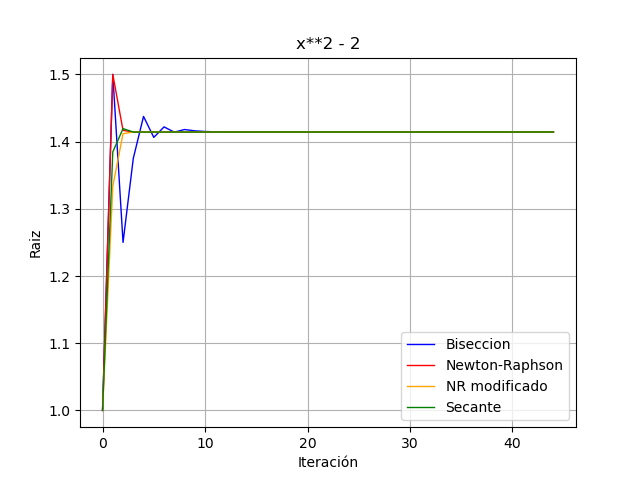
\includegraphics[width=0.8\textwidth]{raiz f1.png}
\caption{\label{fig:class01}Valor de la raíz según iteración.}
\end{figure}
\\
\begin{figure}[H]
\centering
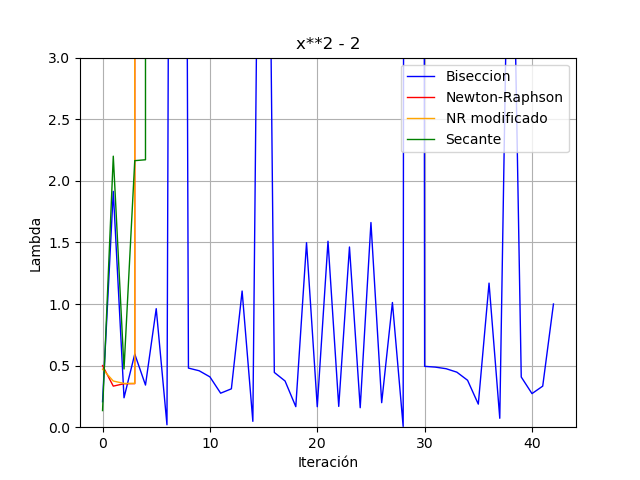
\includegraphics[width=0.8\textwidth]{lambda f1.png}
\caption{\label{fig:class01}Valor de $\lambda$ según iteración.}
\end{figure}
\begin{figure}[H]
\centering
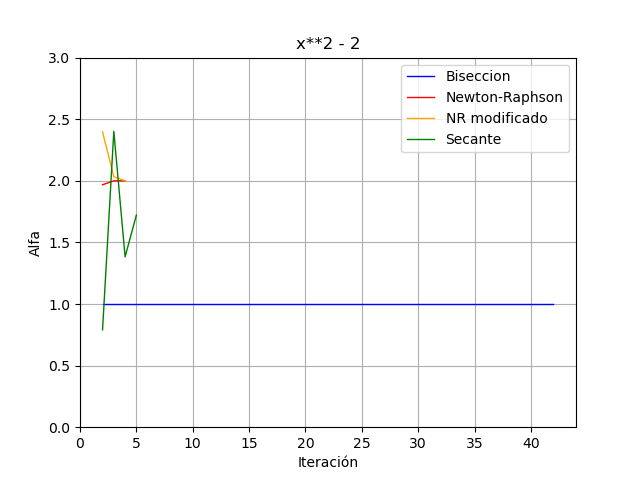
\includegraphics[width=0.8\textwidth]{alfa f1.png}
\caption{\label{fig:class01}Valor de P según iteración.}
\end{figure}
\\Podemos ver como los valores de P están de acuerdo con lo que se esperaba en base a la teoría, mostrando una convergencia lineal para la bisección, una cuadrática para los métodos Newton-Raphson y Newton-Raphson modificado y una convergencia supralineal para el método de la secante.
\subsubsection{Segunda función}\label{sec:CR2}

Usando la biblioteca 'SciPy', las raíces halladas fueron:
\begin{itemize}
    \item[$*$]Usando bisección:   1.2000045776367188+-0.000000000000001
    \item[$*$]Usando Newton Raphson:  1.2000066214794778+-0.000000000000001
\end{itemize}

Los resultados obtenidos con las funciones programadas son congruentes con estos últimos para la tolerancia $1*10^-5$, no así para la cota de error $1*10^-13$, se estima que esto se debe a como esta programado el método de la biblioteca. Para esta función, claramente el método de Newton-Raphson modificado fue el que mostró una convergencia más acelerada. 

\\Analizando la diferencia en iteraciones para las dos cotas de error, se observa que prácticamente necesitaron la misma cantidad.
\begin{figure}[H]
\centering
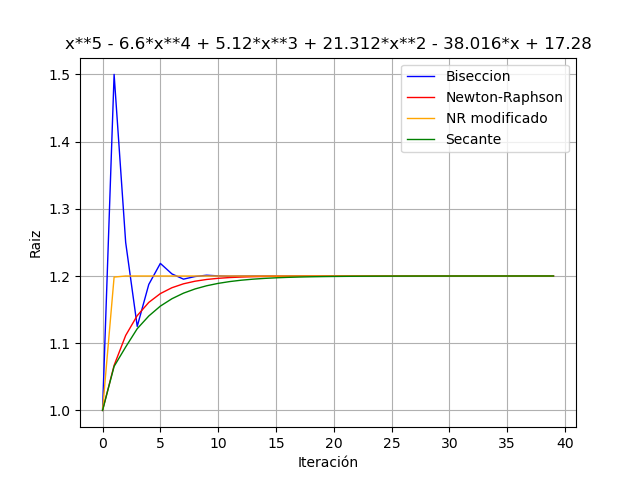
\includegraphics[width=0.8\textwidth]{raiz f2.png}
\caption{\label{fig:class01}Valor de la raíz según iteración.}
\end{figure}
\\
\begin{figure}[H]
\centering
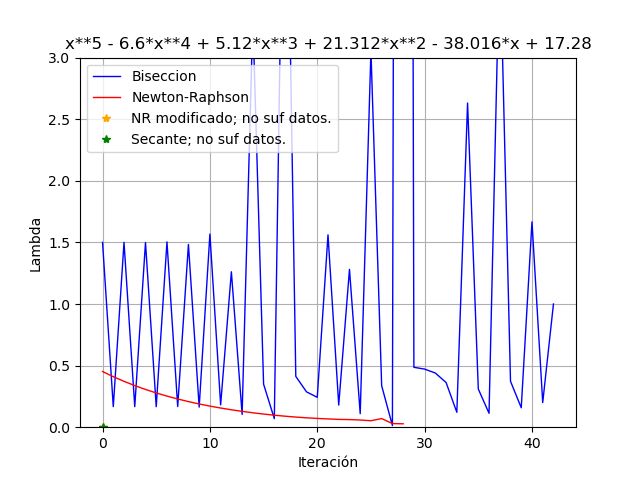
\includegraphics[width=0.8\textwidth]{lambda f2.png}
\caption{\label{fig:class01}Valor de $\lambda$ según iteración.}
\end{figure}
\begin{figure}[H]
\centering
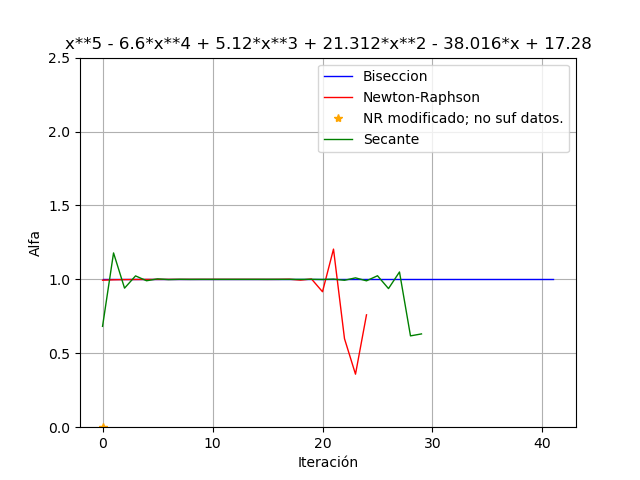
\includegraphics[width=0.8\textwidth]{alfa f2.png}
\caption{\label{fig:class01}Valor de P según iteración.}
\end{figure}
\\%Podemos ver como los valores de P están de acuerdo en lo visto en la teórica, mostrando una convergencia lineal para la bisección, una cuadrática para los métodos Newton-Raphson y Newton-Raphson modificado y 1,6 para el método de la secante.
%falta analizar la parte de lambda, chequear si lo que puse de P está correcto

\subsubsection{Tercera función}\label{sec:CR3}

Usando la biblioteca `SciPy`, las raíces halladas fueron:
\begin{itemize}
    \item[$*$]Usando bisección:   1.500000000000000+-0.000000000000001
    \item[$*$]Usando Newton Raphson:  1.500000000000000+-0.000000000000001
\end{itemize}

Para esta función, la convergencia más rápida fue utilizando el método de bisección, aunque los otros métodos tuvieron también una rápida convergencia. 

\begin{figure}[H]
\centering
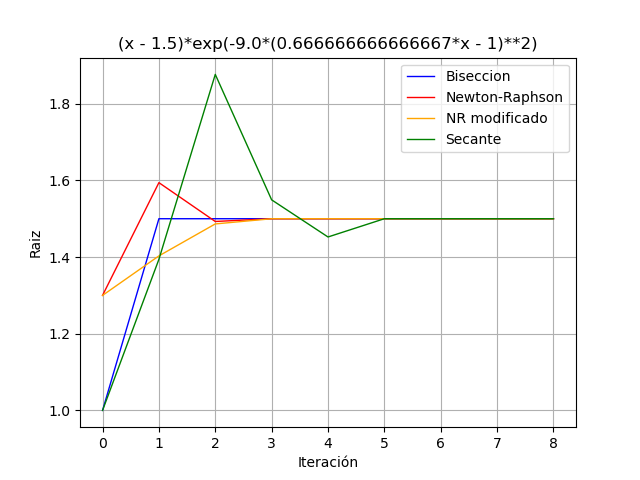
\includegraphics[width=0.8\textwidth]{raiz f3.png}
\caption{\label{fig:class01}Valor de la raíz según iteración.}
\end{figure}
\\
\begin{figure}[H]
\centering
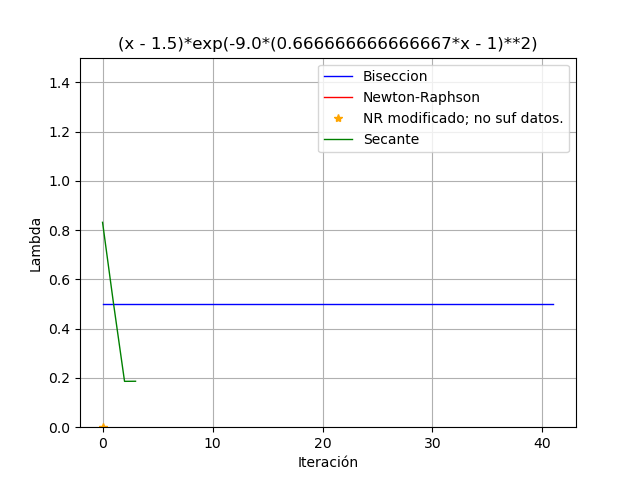
\includegraphics[width=0.8\textwidth]{lambda f3.png}
\caption{\label{fig:class01}Valor de $\lambda$ según iteración.}
\end{figure}
\begin{figure}[H]
\centering
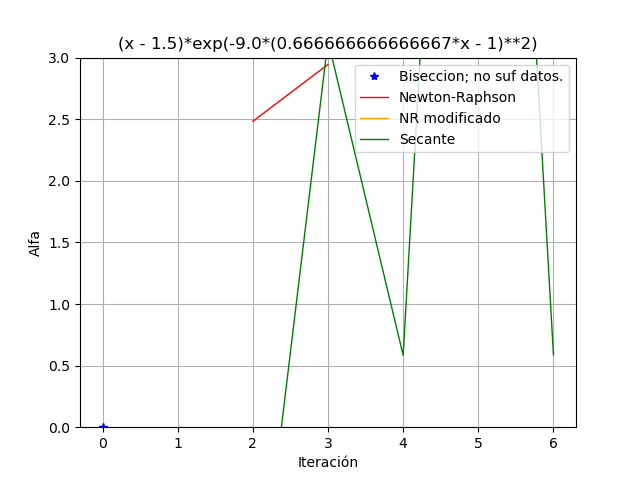
\includegraphics[width=0.8\textwidth]{alfa f3.png}
\caption{\label{fig:class01}Valor de P según iteración.}
\end{figure}
\\%Podemos ver como los valores de P están de acuerdo en lo visto en la teórica, mostrando una convergencia lineal para la bisección, una cuadrática para los métodos Newton-Raphson y Newton-Raphson modificado y 1,6 para el método de la secante.
%falta analizar la parte de lambda, chequear si lo que puse de P está correcto
\section{Conclusiones}\label{sec:conclusiones}

A modo de conclusión de este trabajo práctico, se destaca que para las dos primeras funciones la convergencia al resultado con la tolerancia dada con menos iteraciones fue utilizando el método de Newton-Raphson modificado, de acuerdo a la teória. Para la tercera función, la convergencia más rápida fue con el método de bisección, esto se debió al intervalo dado, que era ideal para hallar dicha raíz.

 \\Además, se encontraron dificultades para hallar el orden de convergencia P y la constante asintótica $\lambda$. Estimamos que una posible fuente de este inconveniente es el error de redondeo proveniente del uso de notación de punto flotante. Además, al trabajar con números muy cercanos entre si, el error tiende a aumentar al dividir por un número muy pequeño o multiplicando por uno muy grande, siendo estos cálculos necesarios para encontrar los valores que necesitamos. Otro posible origen, es el uso de funciones que no están del todo anidadas, que resultan en un aumento de las operaciones a realizar.
 \\Sobre la función 3, con los métodos NR y NR modificado, elegimos modificar la semilla inicial a 1,3, ya que observamos que con la semilla dada era imposible la convergencia (mediante iteraciones encontramos que el intervalo de convergencia es aproximadamente 1,26 < semilla < 1,74). Pensamos en utilizar algunos pasos de bisección para hallar una semilla más adecuada, pero nos encontramos con que en el segundo paso hallaba la raíz, haciendo que el método de NR sea en vano. Por lo tanto, nos pareció la decisión más adecuada elegir una semilla arbitrariamente dentro del intervalo de convergencia hallado.


\end{document}
